%!TEX root=paper.tex

\newpage
% \section{How Is Reader Personalization Being Used?}
\section{How Is Reading Personalization Being Used?}
% \section{How Do Learners Use Reader Personalization?}
% \section{How Do Students Use the Possibility of Reading Personally Interesting Articles?}
\label{sec:results}


% \subsection {Feed Subscriptions}
Figure \ref{fig:subscriptions} represents an incidence matrix in which the columns represent students and the rows represent article sources. If a student is registered to a given source, the intersection of the respective row and column is a $\Diamond$. 
% 
We would expect to see full horizontal rows of data-points if every user subscribed to a given feed, and full vertical rows if every user subscribed to all of the feeds available. The absence of such patterns proves that different individuals prefer to subscribe to different sources.

% The figure illustrates that giving the students the freedom to choose the sources they wanted, allowed each one of them to express their interest. 

\begin{figure}[h!]

\centering
  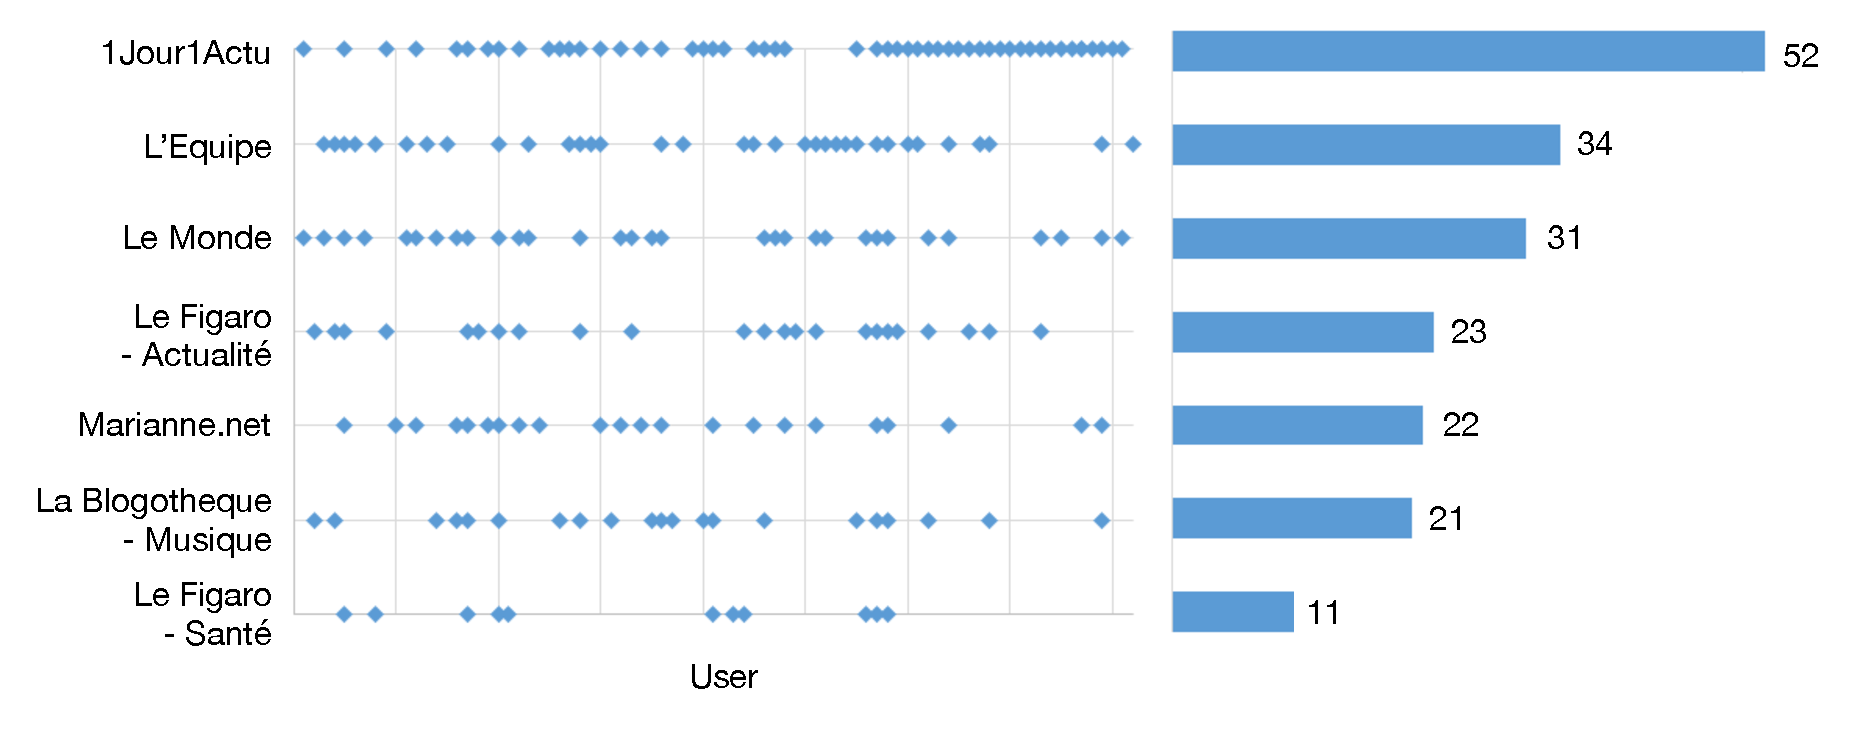
\includegraphics[width=\columnwidth]{figures/subscriptions}
  \caption{Different students subscribe to different sources}
  \label{fig:subscriptions}  
\end{figure}

Projecting the data points onto the horizontal axis results in the histogram to the right of Figure \ref{fig:subscriptions} which shows that source popularity varies. 
% Projecting the data- points onto the horizontal axis and sorting the results results in the histogram in Figure \ref{fig:feedpopularity}.
% 
% \begin{figure}[h!]
% \centering
%   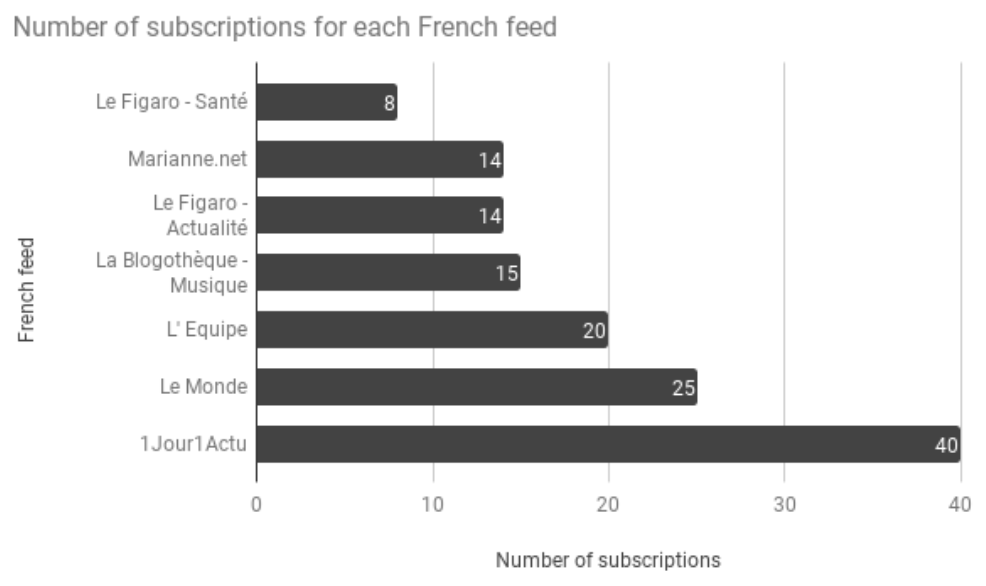
\includegraphics[width=0.85\columnwidth]{figures/feed_popularity}
%   \caption{Some feeds are more popular than others}
%   \label{fig:feedpopularity}
% \end{figure}
% {\em 1Jour1Actu} is the most popular article source and Le Figaro - Sant\'e is the least. 
To show that popularity is not related to the order in which they are presented in the subscription dialog, Figure \ref{fig:popularityvsranking} compares the popularity order with display  order. 
% One can see how the second-to-last presented feed, Le Monde, is the second most popular feed by measure of subscriptions. Conversely, the feed listed above Le Monde is actually the least subscribed-to feed in our listing.


\begin{figure}[h!]
\centering
  %!TEX root=paper.tex
\newcommand{\picscale}{0.45}
\newcommand{\yunit}{0.5}
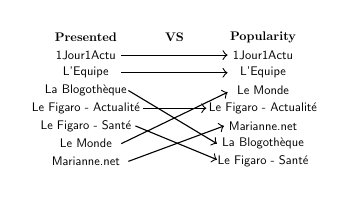
\begin{tikzpicture}[scale=\picscale, every node/.style={scale=\picscale},font=\sffamily]
    % Columns.
    \node at (0  , 0) {\bf Presented};
    \node at (2.5, 0) {\bf VS};
    \node at (5  , 0) {\bf Popularity};
    
    % As presented.
    \node at (0,-1*\yunit) {1Jour1Actu};
    \node at (0,-2*\yunit) {L'Equipe};
    \node at (0,-3*\yunit) {La Blogoth\`{e}que};
    \node at (0,-4*\yunit) {Le Figaro - Actualit\'{e}};
    \node at (0,-5*\yunit) {Le Figaro - Sant\'{e}};
    \node at (0,-6*\yunit) {Le Monde};
    \node at (0,-7*\yunit) {Marianne.net};
    
    % As popular.
    \node at (5,-1*\yunit) {1Jour1Actu};
    \node at (5,-2*\yunit) {L'Equipe};
    \node at (5,-3*\yunit) {Le Monde};
    \node at (5,-4*\yunit) {Le Figaro - Actualit\'{e}};
    \node at (5,-5*\yunit) {Marianne.net};
    \node at (5,-6*\yunit) {La Blogoth\`{e}que};
    \node at (5,-7*\yunit) {Le Figaro - Sant\'{e}};
    
    % Arrows between presented and popular.
    \draw [->] (1,-1*\yunit)   --   (4,-1*\yunit);
    \draw [->] (1,-2*\yunit)   --   (4,-2*\yunit);
    \draw [->] (1.2,-3*\yunit) --   (3.7,-6*\yunit);
    \draw [->] (1.6,-4*\yunit) --   (3.4,-4*\yunit);
    \draw [->] (1.4,-5*\yunit) --   (3.7,-6.9*\yunit);
    \draw [->] (1,-6*\yunit)   --   (4,-3.1*\yunit);
    \draw [->] (1.2,-7*\yunit) --   (3.9,-5*\yunit);
    
\end{tikzpicture} 
  \caption{The popularity of the feeds vs. their ranking in the UI}
  \label{fig:popularityvsranking}
\end{figure}



% \subsection{Article Interactions}
Figure \ref{fig:articles_read} shows an incidence matrix of users (columns) and articles that they interact with (rows). 
The distinct column patterns hint at the fact that each user explores their own interest:
  a few students read exclusively articles about sports (e.g. one student read twelve articles only about sports), 
  one student reads exclusively articles about health;
  nobody reads on all the topics but the majority read on multiple ones.

% , and there is no one article that is interesting for all. 
% The vertical ``line'' in the figure's left half represents an over-active reader.
% \begin{added}
  % Interacting with means that the user translated at least one word in that article. to check with Dan that this is the definition! we currently do not have information about whether a user read the article to the end. 
% \end{added}
% 
% \begin{added}
% 
  % After investigating the reading patterns of students we observed that there are those who enjoy reading a variety of topics, but also those who like to read a single topic. 
  % From the latter category we mention:
 % \cite{renadya07-power}.
  % \begin{itemize}
  %   \item one student who has read twelve articles exclusively on topics about sports in five different days
  %   \item one student who has read six articles exclusively about health topics over two distinct days
  %   \item TODO: Add discussion about some students who have a more omnivorous taste, and thus, also read much more.
  % \end{itemize} 


    % The student \#657 in the published dataset has read 10 articles exclusively about sport in three different days between June 7 and July 4th. 
  
% \end{added}

\begin{figure}[h!]
\centering
  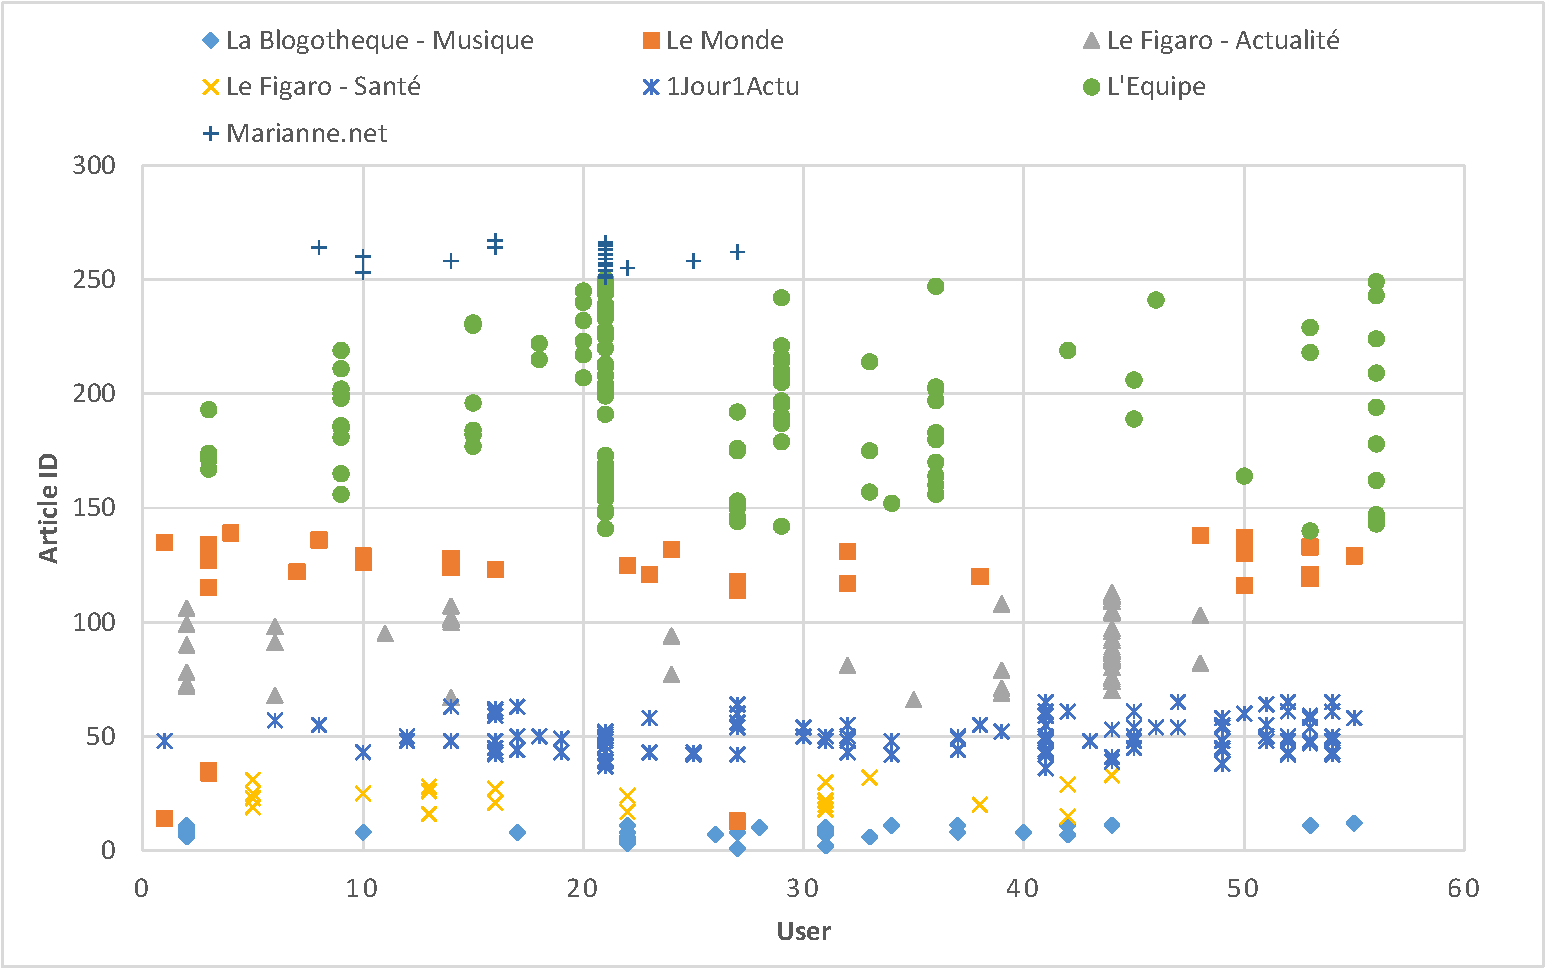
\includegraphics[width=\columnwidth,trim={24 20 40 20},clip]{figures/users_articles_color}
  \caption{Each student (column) reads a different article mix}~\label{fig:articles_read}
\end{figure}
